
\chapter{用户兴趣探索}
\section{引言}
\label{chap:interestExplore}
电子商务产品的设计往往是数据驱动的,即许多产品方面的决策都是把用户行为数据量化后得出的。但就商品而言,那些热门主题往往只代表了用户一小部分的个性化需求,只有通过对用户行为的充分分析,才能更好的挖掘出用户的兴趣,最终提升商品的销售量。现有的推荐算法注重用户或资源间的相似性的同时却忽略了用户兴趣的动态变化,从而导致系统在时间维度上有偏离用户需求的趋势。

为了更好的探索用户兴趣的数据来源包括用户画像和商品特征表。用户画像包括用户基本信息和兴趣标签等,商品特征表包括分类、属性标签等,用户兴趣探索过程分为几个步骤:首先,利用用户历史行为(评论,停留时长,评分,点赞,购买等)量化用户满意度,然后利用用户兴趣特征向量与商品特征矩阵得出相关分数,如果商品与用户的相关分数很低,但有很高的用户满意度,说明是一次成功的用户兴趣探索,更新用户画像。如果是热门商品,大量的用户都会点击,但商品与用户不是很相关,则认为其探索效果是有限的,反之如果是小众商品,考虑到长尾效应,则可以认为其是更成功的兴趣探索。这里涉及到的概念包括用户满意度的量化、用户和商品的关联度、商品属性标签的长尾性。

\section{用户行为数据的存储和处理}
手机主题用户行为数据的特点包括:用户基数庞大。手机主题注册用户达千万级,活跃用户达百万级;用户规模增长快。月新注册用户达10万数量级。每个用户的行为数量较小。即使是活跃用户,每天最多也只产生上百条行为记录;用户行为的计算较为复杂。计算用户的两次登录间隔天数、反复购买的商品、累积在线时间,这些都是针对用户行为的计算,通常具有一定的复杂性;用户行为数据格式不规整,字段丢失率较高。根据用户行为数据的这些特点,我们采用基于HDFS分布式文件集群存储数据。

HDFS为海量的数据提供了存储,则Hive支撑了海量的数据统计。Hive是建立在Hadoop上的数据仓库基础架构。它提供了一系列的工具,用来进行数据提取、转换、加载,是一种可以存储、查询和分析存储在Hadoop中的大规模数据机制。可以把Hadoop下结构化数据文件映射为一张成Hive中的表,并提供类sql查询功能,除了不支持更新、索引和事务,sql其它功能都支持。可以将sql语句转换为MapReduce任务进行运行,作为sql到MapReduce的映射器。提供shell、JDBC/ODBC、Thrift等接口。优点是成本低可以通过类sql语句快速实现简单的MapReduce统计。从体系架构到数据定义到数据存储再到数据处理,HDFS分布式文件集群和Hive为海量用户行为的分析和用户兴趣探索提供了可能。
  \subsection{数据预处理}
  数据预处理是数据挖掘过程中一个重要步骤,主要工作包括字段去重、无效日志过滤、多表字段的连接等。如统计2015年09月06号userId为001的投诉数,数据预处理过程:
  \begin{lstlisting}
    set hiveconf:ymdwithline=2015-09-06;
    set hiveconf:metric=complaint_order_num;
    set hiveconf:user_id=001;

    select '${hiveconf:metric}' as metric, count(a.order_id) as score
    from (
        //去重
        select distinct order_id
        from theme.dw_v_order_base
        //以时间范围date_sub('${hiveconf:ymdwithline}',5) and '${hiveconf:ymdwithline}'为条件过滤掉不符合条件的订单
        where concat_ws('-',year,month,day) between date_sub('${hiveconf:ymdwithline}',5) and '${hiveconf:ymdwithline}'
        //无效订单过滤
        and order_id!=null
        //以用户id为条件过滤掉其他订单
        and user_id=${hiveconf:user_id}
    ) a
    inner join (
        //order_id 字段去重
        select distinct order_id
        from theme.g_comment_complaint
        //type = 3表示用户投诉
        where concat_ws('-',year,month,day) = '${hiveconf:ymdwithline}' and type = 3
        //多表字段的连接,如果有一个表有投诉记录,就算一次投诉。
        union
        select distinct order_id
        from theme.dwd_kefu_phone_complaint
        where concat_ws('-',year,month,day) = '${hiveconf:ymdwithline}'
    ) b
    on a.order_id = b.order_id
    inner join (
        select order_id
        from theme.pay_info
        where ymd = ${hiveconf:ymdwithline}
            //status=1代表当前订单状态为已支付
            and status=1
    ) d
    on a.order_id = d.order_id
    group by metric;
  \end{lstlisting}

\section{用户兴趣探索模型}
用户兴趣探索主要功能模块包括:1,兴趣标签探测,在分析用户行为数据时,如果某些主题标签是这个用户画像没有的,那么这些标签会作为标签探索候选集。2,长尾标签提取,遍历标签探索候选集,如果不属于小众标签集的标签将会被过滤掉。3,用户满意度量化,根据用户所有对某一个主题的行为数据得出这个用户对这个主题的满意度。4,标签权重的更新,不管是不是一次成功的兴趣标签探索,都要对用户画像标签的权重做更新,更新算法利用了线性衰减思想。本章首先介绍一些基本概念,包括长尾标签的定义、用户满意度的量化等。然后详细介绍用户兴趣探索功能模块的实现。
  \subsection{基本概念概述}
  实体域。当我们想基于用户行为分析来建立用户兴趣模型时,我们必须把用户行为和兴趣主题限定在一个实体域上。个性化推荐落实在具体的推荐中都是在某个实体域的推荐。对于手机主题应用市场来说,实体域包括所有的主题,背景图片,铃声,闹铃等。

  用户行为。包括浏览,点击,下载,试用,购买,评论。本文所指的用户行为都是指用户在某手机主题上的行为。
  
  用户兴趣。用户兴趣同样是限定在某实体域的兴趣,通常以标签+权重的形式来表示。比如,对于手机主题,用户兴趣向量可以是「动漫,0.6」,「NBA,0.1」,「性感,0.7」等分类标签。值得一提的是,用户兴趣只是从用户行为中抽象出来的兴趣维度,并无统一标准。而兴趣维度的粒度也不固定,如「体育」,「电影」等一级分类,而体育下有「篮球」,「足球」等二级分类,篮球下有「NBA」,「CBA」,「火箭队」等三级分类。我们选取什么粒度的兴趣空间取决于具体业务模型。

  兴趣空间。用户兴趣是在同一层次上兴趣维度的集合,比如手机主题中,可以用「热门」,「游戏」,「限时特价」,「科技」来构成一个程序员兴趣标签空间,也可以用「二次元」,「萝莉」,「魔幻」,「纯真」,「召唤兽」·····「法术」等构成一个动漫兴趣标签空间。

  小众标签集。小众标签集是指出现频率低的主题标签的集合,代码:
  \begin{lstlisting}
    public HashSet<String> getLongTailTags() throws Exception {
        Map<String, String> tagsCount = new TreeMap<>();

        //获取所有主题包
        Map<String, Object> allThemes = getAllThemes();
        for (Map.Entry<String, Object> theme : allThemes.entrySet()) {
            String themeName = theme.getKey();
            //获取当前主题的所有标签
            Object themeTags = ((Map<String, Object>) theme.getValue()).get("tags");
            for (String tag : (Set<String>) themeTags) {
                //出现一次,tag 对应的count加1
                tagsCount.put(tag, tagsCount.get(tag) + 1);
            }
        }

        //这里将map.entrySet()转换成list
        List<Map.Entry<String, String>> list = new ArrayList<Map.Entry<String, String>>(tagsCount
                .entrySet());
        //然后通过比较器来实现排序
        Collections.sort(list, new Comparator<Map.Entry<String, String>>() {
            //升序排序
            public int compare(Map.Entry<String, String> o1, Map.Entry<String, String> o2) {
                return o1.getValue().compareTo(o2.getValue());
            }
        });

        HashSet<String> out = new HashSet<>();
        //取频率最小的那80%标签作为小众标签
        double threshold = list.size() * 0.8;
        for (int i = 0; i <= threshold; i++) {
            out.add(list.get(i).getKey());
        }

        return out;
    }
  \end{lstlisting}

  用户满意度量化。用户满意度量化是指根据用户作用在主题上的不同行为动作及其参数值,参数值包括动作类型、次数和时长,得到一个衡量用户满意度的分数。

  标签集中度(tagFocus)。标签集中度是指如果某个标签在一类主题中出现的频率高,其他主题类型很少出现,则认为此兴趣标签具有很好的类别区分能力。这是因为包含兴趣标签t的主题越少,也就是n越小,则说明标签t具有很好的兴趣区分,则其探索权重越大。如果某一类主题包C中包含兴趣标签t的个数为tagInThemeNum,而其它类包含t的总数为tagInOtherNum,则所有包含t的主题数n=allThemeNum,当m大的时候,n也大,标签权重值会小,就说明该标签t类别区分能力不强。实际上,如果一个标签在一个类的主题中频繁出现,则说明该标签能够很好代表这类主题的特征,这样的标签应该给它们赋予较高的权重,并选来作为该类主题的特征向量以区别于其它类主题,标签集中度公式如\autoref{equ:focus},我们很容易发现,如果一个标签只在很少的主题包中出现,我们通过它就容易锁定搜索目标,它的权重也就应该大。反之如果一个词在大量主题包中出现,我们看到它仍然不很清楚要找什么内容,因此它应该权重较小。
  \begin{equation}
    tagFocus=log\frac{|tagInThemeNum|}{|allThemeNum|}
    \label{equ:focus}
  \end{equation}


  标签热度(tagPopular)。标签热度指的是某一个给定标签在用户画像中出现的频率。例如在300万用户总数中,十分之一的用户标签中有"火影"标签,那么其热度为0.1,除此之外有些标签如"精品","气质"等标签占了总词频的80\%以上,而它对区分主题类型几乎没有用。我们称这种词叫“应删标签”。即应删除词的权重应该是零,也就是说在度量相关性是不应考虑它们的频率。热度公式如\autoref{equ:hot}。
  \begin{equation}
    tagPopular=log\frac{|peopleLikeTagNum|}{|allPeople|}
    \label{equ:hot}
  \end{equation}

  \subsection{兴趣标签探测功能模块}
  首先候选标签是用户画像中没有的标签,如用户001每次都会浏览动漫、美少女主题,但是有一天却购买了一款汽车手机主题,那么程序可以检测汽车标签对于用户001是从未遇到过的标签,于是汽车标签将会是潜在的探索标签。事实上用户兴趣探索过程可以在很短的时间内完成,基于 hive + HDFS 平台的时长维度为天,而基于 kafka + spark 平台可以将时长维度降到小时级别。标签探索算法:
  \begin{lstlisting}
    public Set<String> tagExplore(String userId, String itemId) throws Exception {
        Gson gson = new Gson();
        //获取当前用户对当前主题的所有行为,只计算前一天的行为
        List<UserActions> actions = getActionsByUserIdAndItemId(userId, itemId);
        //获取用户详细信息
        String userInfo = getUserBaseInfo(userId);
        UserProfile userProfile = gson.fromJson(userInfo, UserProfile.class);
        Map<String, Double> userTags = userProfile.tags;

        Set<String> out = new HashSet<>();
        for (UserActions action : actions) {
            //获取主题详细信息
            Map<String, Object> itemBaseInfo = getItemBaseInfo(action.itemId);
            Set<String> tags = (Set<String>) itemBaseInfo.get("tags");
            for (String tag : tags) {
                if (!userTags.containsKey(tag)) {
                    out.add(tag);
                }
            }
        }
        return out;
    }
  \end{lstlisting}

  \subsection{长尾标签抽取功能模块}
  长尾标签是指这个标签的集中度和热度之比大于一个阈值,且在小众标签集中。长尾标签提取算法。
  \begin{lstlisting}
    public Set<String> getEffectTags(String userId, String itemId) throws Exception {
        Set<String> out = new HashSet<>();
        //获取所有长尾标签
        HashSet<String> longTailTags = getLongTailTags();
        //获取所有当前用户画像没有的标签
        Set<String> rawTags = tagExplore(userId, itemId);
        for (String tag : rawTags) {
            if (!longTailTags.contains(tag)) {
                continue;
            }

            //获取标签的集中度
            long tagFocusScore = getTagFocusScore(tag);
            //获取标签的热度
            long tagPopularScore = getTagPopularScore(tag);
            if (tagFocusScore / tagPopularScore <= threshold) {
                continue;
            } else {
                out.add(tag);
            }
        }

        return out;
    }
  \end{lstlisting}

  \subsection{用户满意度量化功能模块}
  从对用户的行为数据分析量化用户满意度,并基于此实现兴趣标签探索,如何收集用户的偏好行为成为用户兴趣探索效果最基础的决定因素。用户有很多方式向系统提供自己的偏好信息,而且不同的应用也可能大不相同。
  \autoref{tab:userAction}列举的用户行为为实际使用的行为类型,根据不同行为反映用户喜好的程度将它们进行加权,得到用户对于物品的总体喜好。显式的用户反馈比隐式的权值大,但比较稀疏,毕竟进行显示反馈的用户是少数;而隐式用户行为数据是用户在使用应用过程中产生的,它可能存在大量的噪音和用户的误操作,通过数据挖掘算法过滤掉行为数据中的噪音,这样使分析更加精确。然后是归一化操作,因为不同行为的数据取值可能相差很大,比如,用户的浏览数据必然比购买数据大的多,如何将各个行为的数据统一在一个相同的取值范围中,从而使得加权求和得到的总体喜好更加精确,就需要进行归一化处理使得数据取值在 [0,10] 范围中,代码:
  \begin{lstlisting}
    public Map<String, String> getUseSatisfyScore(String userId, String itemId) {
        //获取当前用户对当前主题包的所有行为
        List<UserActions> actions = getActionsByUserIdAndItemId(userId, itemId);
        double score = 0.0;
        int clickNum = 0;
        int scrollNum = 0;
        for (UserActions action : actions) {
            if (action.actionType.equals("buy") || action.actionType.equals("tryUse") || action
                    .actionType.equals("favor")) {
                return new HashMap<String, String>() {{
                    put("score", "1");
                    put("msg", "very like");
                }};
            } else if (action.actionType.equals("down")) {
                return new HashMap<String, String>() {{
                    put("score", "0");
                    put("msg", "not like at all");
                }};
            } 

            if (action.actionType.equals("click")) {
                clickNum++;
                if (clickNum <= 5) {
                    score += 0.2;
                }
            } else if (action.actionType.equals("scroll")) {
                scrollNum++;
                //滑动屏幕一次且停留时长超过3秒,说明用户对内容感兴趣
                if (scrollNum <= 5 && action.duration * 1000 > 3000) 
                    score += 0.5;
            } else if (action.actionType.equals("share")) {
                score += 1.5;
            } else if (action.actionType.equals("comment")) {
                score += 1.0;
            } else if (action.actionType.equals("star")) {
                //用户评分,值为1到5星
                if(action.starLevel>=4)
                  score += action.starScore;
            }
        }

        //正则化
        score = (score-MIN)/(MAX-MIN)
        HashMap<String, String> ret = new HashMap<>();
        ret.put("score", String.valueOf(score));
        ret.put("msg", "user intereting in this item");
        return ret;
    }
  \end{lstlisting}

    \begin{table}[htp]
    \centering
    \tabcaption{用户行为权重对应表}
    \label{tab:userAction}
    \begin{tabular}{ |c|c|p{4cm}|p{5cm}|c|} \hline
     用户行为 & 类型 & 特征 & 作用 & 权重\\ \hline
     评分 & 显式 & 整数量化的偏好,可能的取值是 [0,5] & 通过用户对物品的评分,可以精确的得到用户的满意度,但是噪声比较大,比如遇到好评返现活动 & 1\\ \hline
     分享 & 显式 & 布尔量化的偏好,取值是 0 或 1 & 通过用户对物品的投票,可以精确的得到用户的喜好度,同时可以推理得到被转发人的兴趣取向 & 2\\ \hline
     评论 & 显式 & 一段文字,需要进行文本分析,得到偏好 & 通过分析用户的评论,可以得到用户的情感:喜欢还是讨厌 & 1\\ \hline
     赞/踩 & 显示 & 布尔量化的偏好,取值是 0 或 1 & 带有很强的个人喜好度 & 3 \\ \hline
     购买、试用 & 显式 & 布尔量化的偏好,取值是 0 或 1 & 用户的购买是很明确的说明这个项目它感兴趣。& 3 \\ \hline
     点击流 & 隐式 & 包括滑屏频率,滑屏次数,屏停留时长,用户对物品感兴趣,需要进行分析,得到偏好 & 用户的点击一定程度上反映了用户的注意力,所以它也可以从一定程度上反映用户的喜好。& 1 \\ \hline
     停留时长 & 隐式 & 一组时间信息,噪音大,需 要进行去噪,分析,得到偏 好 & 用户的页面停留时间一定程度上反映了用户的注意力和喜好,但噪音偏大,不好利用。比如说用户在浏览一个主题的时候,丢下手机和同学出去踢球去了,页面提留时长可能会很长 & 1 \\ \hline
    \end{tabular}
    \end{table}

  \section{用户画像和用户兴趣探索的融合}
  随着时间的变化,用户的兴趣会发生转移,时间越久远,标签的权重应该相应的下降,距离当前时间越近的兴趣标签应该得到适当突出。出于这样的考虑,一般会在标签权重值上叠加一个时间衰减函数,这个时间衰减函数被设计成、的形式,通过定义衰减幅度和周期,调节衰减的程度,体现不同的时效性。
  我们可以把用户画像权重想象成一个自然冷却的过程:
  \begin{itemize}
    \item 任一时刻,用户画像中的标签都有一个当前温度,温度最高的标签权重值最高。
    \item 如果该用户对某主题发生了一些正向标签,如点赞,该文章包含的标签在用户画像中的温度就会上升,否则温度下降。
    \item 随着时间流逝,所有标签的温度都逐渐冷却。
  \end{itemize}

  这样假设的意义在于我们可以照搬物理学的牛顿冷却定律(\href{http://www.evanmiller.org/rank-hotness-with-newtons-law-of-cooling.html}{Newton's Law of Cooling}),建立标签权重与时间之间的函数关系:本期分数 = 上期分数 - 冷却系数$*$间隔天数,构建一个线性衰减的过程。其中,冷却系数决定了标签融合的更新率,如果想放慢更新率,冷却系数就取一个较小的值,否则就取一个较大的值。

  标签权重的线性衰减算法结合了手机主题用户长期兴趣和短期兴趣,根据时间因素权重自动进行衰减,能准确反映用户兴趣的变化趋势。该模型是指用户对兴趣标签的评分仅代表评价当时的兴趣度,随着时间的推移,用户对该资源项目的评分将规律性地自动衰减,当项目评分衰减到 0 时,该标签将被用户画像所淘汰。
  \begin{lstlisting}
      public void tagLinearecay(String userId) throws Exception {
        //获取当前用户当前所有有过行为的主题包
        Set<String> items = getAllItems(userId);
        //获取当前用户的画像
        UserProfile userProfile = getUserProfile(userId);
        for (String item : items) {
            //获取当前用户对当前标签的满意度值
            Map<String, String> useSatisfyScore = getUseSatisfyScore(userId, item);
            //threshold为逻辑回归算法训练出的阈值
            if (Double.parseDouble(useSatisfyScore.get("score")) > threshold) {
                //获取所有成功探索的标签
                Set<String> effectTags = getEffectTags(userId, item);
                for (String effectTag : effectTags) {
                    userProfile.tags.put(effectTag, 5);
                }
            }
        }
        //得到用户行为中所有的主题标签
        Set<String> allActionTags = getAllActionTags(userId);
        for (Map.Entry<String, Double> userTag : userProfile.tags.entrySet()) {
            String tag = userTag.getKey();
            double score = userTag.getValue();
            if (!allActionTags.contains(tag)) {
                //将标签偏好值减少 0.5,进行衰减。
                score -=0.5;
                if(score<=0){
                    //如果当前标签权重降低0以下,则移除该标签
                    userProfile.tags.remove(tag);  
                }else {
                    userProfile.tags.put(tag, score);
                }
            }else {
                //do nothing
            }
        }
    }
  \end{lstlisting}


\section{实验与分析}
  \subsection{数据集准备}
  实验中我们利用2003年9月到2003年10月的用户行为数据和所有关联的手机主题包。这个数据集包含了110739个用户在这段时间对主题包的标签行为,数据集中包含了8936个主题包。该数据集每行是一条记录,每条记录由四个部分组成:用户ID,行为类型,行为属性值,主题ID,日期,每一条记录代表了某个用户在某个时间点对某个主题包进行了某种行为。保证数据集具有一定的稠密程度,我们去除了用户行为记录少于10条的所有用户,最终用户集包含10646个用户,2033600条用户行为记录,可见数据集的稀疏度还是在97.86\%以上。
  \subsection{评测指标}
  使用线上A/B测试方案,利用点击购买转化率来评测推荐系统应对马太效应的效果\citep{matthew-effect}。根据统计我们知道20\%的热门商品在占了80\%的曝光机会的同时却只占50\%的销售量,这时因为虽然热门商品销量很好但其整体数量偏少,很难满足大多数消费者的需求。相反,占据80\%的小众商品虽然曝光率低,但凭借其庞大数量和多样性,可以满足不同消费者的需求。因此如果适度对小众商品增加曝光机就会可以提升所有商品的销售量,即提升手机主题包的点击购买转换率。
  \subsection{对比模型}
  无兴趣探索模块的推荐模型,在实验中作为基准模型。对照模型包括融合了兴趣探索模块的推荐模型和推荐热门商品的简单推荐模型。
  \subsection{实验结果}
  我们对比了无兴趣探索模块的推荐模型、推荐热门商品的简单推荐模型和融合了兴趣探索模块的推荐模型在2015年9月到2015年10月的有过至少一次销售记录的商品数itemCount。\autoref{pic:hl_themeNumber}展示了不同模型的实验结果。图中,横坐标是时间变量,单位为天,纵坐标是itemCount,每一条曲线代表了一个模型的itemCount随时间变化的曲线。通过观察曲线可知,融合了兴趣探索模块的推荐模型的itemCount月平均数是3136,推荐热门商品的简单推荐模型的itemCount月平均数是1935,无兴趣探索模块的推荐模型的itemCount月平均数是2679。实验说明融合了用户兴趣探索的推荐模型相对其他模型有更好的多样性。
  \begin{figure}
  \centering
    \framebox{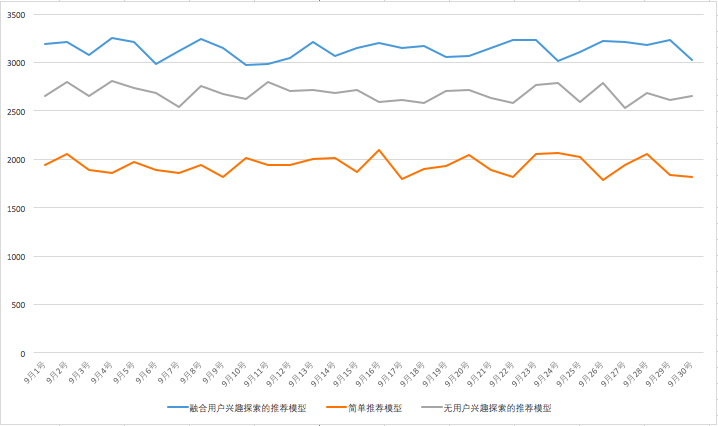
\includegraphics[scale=0.55]{figures/hl_themeNumber}}
    \figcaption{推荐多样性实验对比图}
    \label{pic:hl_themeNumber}
  \end{figure}

  我们对比了无兴趣探索模块的推荐模型、推荐热门商品的简单推荐模型和融合了兴趣探索模块的推荐模型在2015年9月到2015年10月的点击购买转化率。\autoref{pic:hl_buyLookRatio}展示了不同模型的实验结果。图中,横坐标是时间变量,单位为天,纵坐标是点击购买转化率,每一条曲线代表了一个模型的点击购买转化率随时间变化的曲线。实验结果显示,融合了兴趣探索模块的推荐模型相对其他模型有更高的点击购买转化率。融合了兴趣探索模块的推荐模型的平均点击购买转化率是32.74\%,比推荐热门商品的简单推荐模型的平均点击购买转化率9.63\%高了23.11个百分点,相对于无兴趣探索模块的推荐模型的平均点击购买转化率17.54\%高了15.2个百分点。由此可见用户兴趣探索能够很好的提升点击购买转化率。
  \begin{figure}
  \centering
    \framebox{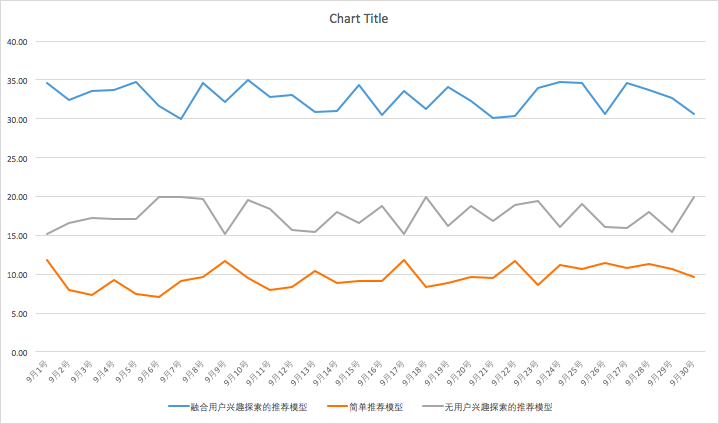
\includegraphics[scale=0.55]{figures/hl_buyLookRatio}}
    \figcaption{转化率实验对比图}
    \label{pic:hl_buyLookRatio}
  \end{figure}

\section{本章小结}
这一章主要研究了标签动态变化的对推荐系统的影响,实际中用户同时会受到社会因素和个人因素的影响,但这两种因素在会产生不同强度的影响。在快速变化的系统中,用户行为更加会受到社会因素的影响,而在变化相对较慢的系统中,用户行为则更加受到个人因素的影响。本章首先介绍了用户行为数据的存储方式以及基于此的用户行为数据的的预处理。然后介绍了用户兴趣探索模块的组成内容,包括兴趣标签探测功能模块、长尾标签抽取功能模块、用户满意度量化功能模块,然后介绍了用户画像和用户兴趣探索的融合,最后给出了用户兴趣探索实验结果。